\chapter{Bevezetés}

Konzulensem, Dr. Szegletes Luca már régóta gyűjt videokártyás kódimplementációkat különböző NP-nehéz problémákra. Amikor megbeszéltük, hogy mi lenne a munkám célja, különböző útkeresési algoritmusok megvalósítását kaptam feladatul. A járműútvonal-tervezési algoritmusoknak nagyon sok alesete van, ugyanis végtelenül sokféle feltételt szabhatunk meg egy bejárás számára: a teljes hossz legyen rövid, az egyes utak legyenek egyenként rövidek, stb. Különböző alkalmazásokhoz nagyon változatos elvárások illenek: például ha egy bútor szállítmányozási cég akarja megtervezni, hogy az aznapi 20 klienséhez milyen sorrendben juttassa el az árukat, már azt is bele kell kalkulálnia, hogy hogyan fognak a termékek elférni egy kamionban (véges kapacitás problémája). Másik példa egy nemzetközi körutazás: a cég vezérigazgatója be szeretné járni egy kampány keretében a cég különböző leányvállalatait, melyek manapság a világ bármely pontján lehetnek: lehet, hogy az egyik üzem Kolumbia közepén, míg egy másik valahol Indiában van. A két ország időzónája nagyon különböző, ezért nem mindegy, hogy az igazgató a nap melyik órájában szeretne találkozni a helyi vezetőkkel (a kliens nem áll korlátlanul rendelkezésre, igazítani kell a fogadó és vendég beosztását). Számtalan hasonló szituáció képzelhető el, a fent említettek csak a legtipikusabbak. Ezen problémákat a számítástudomány már évtizedek óta aktívan kutatja. 

\begin{figure}[ht!]
	\centering
	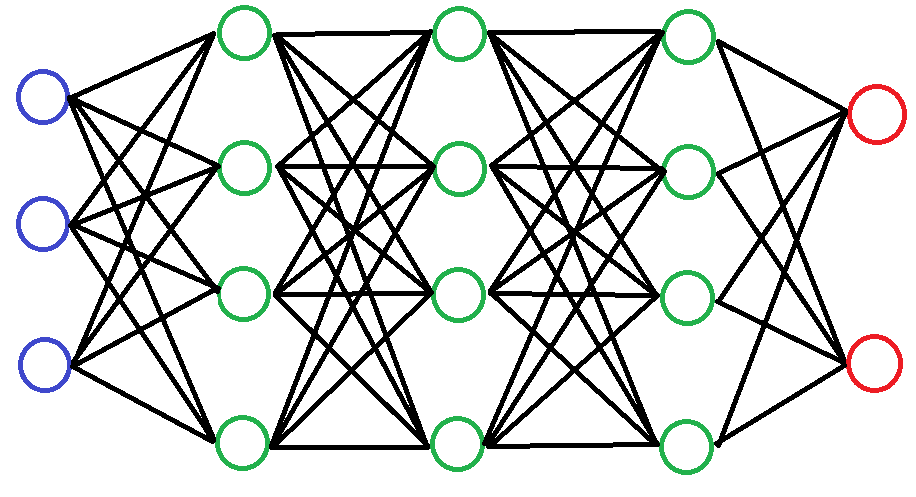
\includegraphics[width=150mm, keepaspectratio]{figures/neurons.png}
	\caption{Többféle modellt is kitaláltak már gépi tanuláshoz, az egyik leghíresebb az ún. neuronháló modell }
\end{figure}
Napjainkban a mesterséges intelligencia forradalmasította a számítástechnikát a számítási kapacitások soha eddig nem látott bővülése eredményeképpen. Az NVIDIA egy olyan cég, amely hardvergyártóként, videokártyák gyártásával és értékesítésével kezdte működését. Az elmúlt években komoly szerkezetváltozáson ment keresztül, igyekszik némileg közönséget is váltani: korábban a videokártyák legnagyobb felvevőpiaca a videojátékosok voltak. A GPU arra lett kitalálva, hogy különböző 2D-, 3D-s renderelési feladatokban tehermentesítse a CPU-t. Több ezer (fizikai) szálon képes futni. Egy GPU szál ezzel szemben sokkal szűkebb utasításkészleten tud dolgozni, mint egy CPU szál. A GPU szálak elsősorban különböző aritmetikai utasítások végrehajtásában jeleskednek: rendelkeznek hardveres FPU-val (floating point unit - olyan hardver, mely lebegőpontos számokon végzett aritmetikára lett tervezve). 
A mesterséges intelligenciát használó algoritmusok azért lettek forradalmi vívmányok, mert az algoritmus kiötletelésének nehézségeit nagyrészt képes kivenni a programozók kezéből. Egy klasszikus módon megírt program írása során a kódírónak teljes körű elképzelése kell, hogy legyen arról, hogy hogyan fog eljutni az eredményhez. 



\begin{figure}[ht!]
	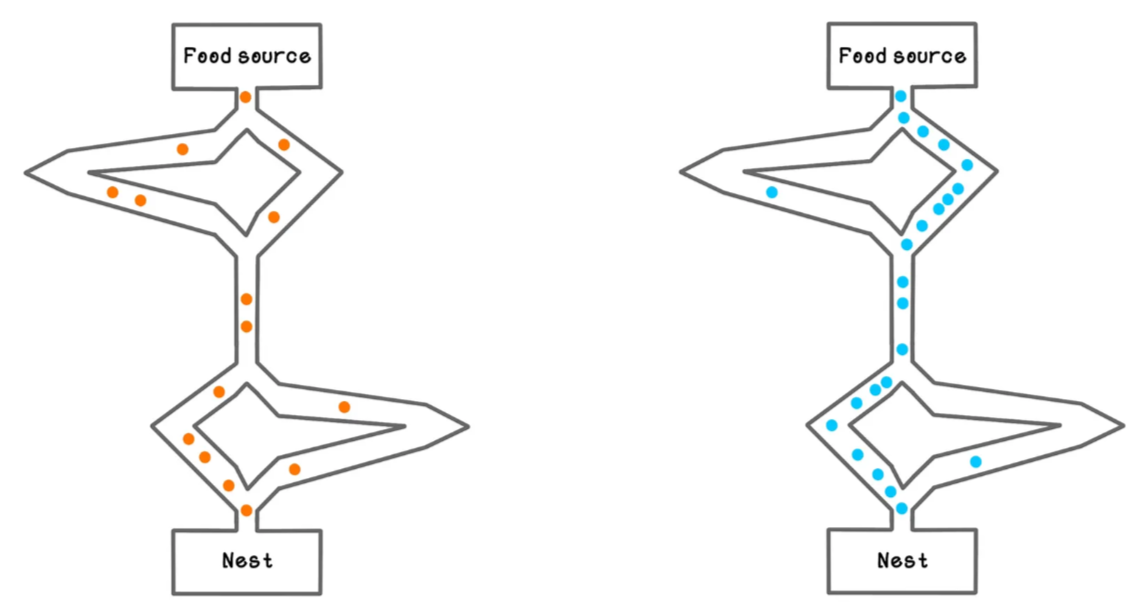
\includegraphics[width=150mm, keepaspectratio]{figures/aco-visualization.png}
	\caption{A hangyák sajátos módon optimalizálják a táplálékszerzést: a Hangyakolónia Optimalizáció segítségével \cite{ACOimage} \label{ACOvisulabel}}
\end{figure}
A gépi tanulás másképp működik: az én esetemben, a \textbf{genetikus algoritmusoknál} kell hozzá egy input, és egy hibafüggvény. A programozó megadja, hogy mely bemenetre szeretné ráengedni az algoritmust. Az algoritmus kap még egy kiértékelő függvényt, amellyel számszerű eredményt rendelhet az általa alkotott megoldásokhoz. A gépnek van memóriaterülete, amelyet az alapján írhat, hogy mit tanult. A genetikus algoritmusok megoldásgenerációkat hoznak létre. A gép a hibafüggvény segítségével értékeli az egyes genomokat, majd a legjobban sikerült egyedek alapján készít következő generációt. A folyamat többféle módon is véget érhet:
\begin{itemize}
	\item a hibafüggvény egy adott hibahatáron belüli megoldást talál
	\item az algoritmus adott ideig (pl. 2 óra) fut, a végső megoldás az utolsó generáció legjobb megoldása
	\item a program adott számú iterációt hajt végre, a végső megoldást készítheti külön, a korábban tanultak alapján
\end{itemize}

A gép kiveszi a programozó kezéből az algoritmizálási feladatot. A kódoló választ egy modellt, amely alapján a gép majd dolgozik. Ha elégedetlenek vagyunk, választhatunk másik modellt, hátha az sikeresebbnek bizonyul.

Szakdolgozatom során a \textbf{Hangyakolónia optimalizáció} modelljét alkalmaztam. Ez egy természetből ellesett trükkön alapuló gráfbejárási algoritmus, a hangyák élelemkeresési módszereire hasonlít, melyet a \ref{ACOvisulabel}. ábra szemlélet.

A koncepció központi elemei a \textbf{feromonok}, melyek biokommunikációra szolgáló, különböző állatok, rovarok által kibocsátott kémiai anyagok, amelyek a faj másik egyedéből meghatározott viselkedést váltanak ki.

A hangyák egész nap a hangyaboly környékét járják morzsák, elhullott rovarok után kutatva. Amikor egy dolgozó korábban felfedezetlen élelemforrást talál, kis részével visszaindul a bolyba, és a hazaúton egyfajta testnedvet, \textbf{feromont} bocsát ki magából. A többi hangya megérzi a szagot, és a nyomába ered. Ha tényleg táplálékhoz vezetett a feromoncsík, akkor ők is kis részével visszaindulnak az élőhelyükre. A folyamat egészen addig tart, amíg van mit elvinni. Ezután az utólag érkező hangyák azt tapasztalják, hogy elfogyott a táplálék, ezért a visszaúton nem választanak ki feromont. A szél előbb-utóbb elfújja az úton hagyott kémiai anyagokat, ezért nem megy oda több egyed.

\section{Áttekintés}
Bevezetés után a \ref{theoryChapter}. fejezetben először ismertetem a problémák elméleti hátterét. Matematikailag kimondom a feladatokat, valamint bemutatom, milyen - főleg valószínűségszámítási - alapok szükségesek a Hangyakolónia optimalizáció alapos megértéséhez.

A \ref{technologyChapter}. fejezetben bemutatom a GPU programozás technológiai hátterét. Kimondom a GPGPU fogalmát. Példákon keresztül szemléltetem a CUDA szoftvermodell markánsabb fogalmait. Különbséget teszek az egyes szinkronizálási szintek között. Ezek után lépésenként megmutatom, hogyan kell Visual Studio segítségével CUDA programot írni és futtatni.

A \ref{implementationChapter}. fejezetben a kódimplementációimat veszem górcső alá. Részletesen beszámolok az egyes logikai elemek működéséről. Bemutatom a Hangyakolónia Algoritmus megjelenését, és az attól való bizonyos eltéréseket. Részletezem a feromonok nyilvántartását, és a véletlen számok kezelését. Logikailag egymásra építem az algoritmusokat ilyen sorrendben: TSP, VRP, CVRP, CVRPTW.

A \ref{resultsChapter}. fejezet a mérési eredményeimet tartalmazza táblázatos formában. Igyekeztem minél szélesebb körben lemérni az egyes adathalmazokat. 

A \ref{results_section}. fejezetben röviden értékelem a kapott eredményeket grafikonokkal szemléltetve. 

\section{Rövidítések}
Dolgozatomban az alábbi rövidítéseket használom:
\begin{itemize}
	\item \textbf{ACO} - Ant Colony Optimization: Hangyakolónia optimalizáció/algoritmus
	
	\item \textbf{CPU} - Central Processing Unit - Processzor
	\item \textbf{CUDA} - Compute Unified Device Architecture
	\item \textbf{CVRP} - Capacitive Vehicle Routing Problem: Korlátozott kapacitású járművek útvonaltervezési problémája
	\item \textbf{CVRPTW} - Capacitive Vehicle Routing Problem with Time Windows: Korlátozott kapacitású, kötött időbeosztású járművek útvonaltervezési problémája
	\item \textbf{FPU} - Floating-point Unit
	\item \textbf{GPU} - Graphics Processing Unit - videokártya
	\item \textbf{OS} - Operating System - Operációs rendszer
	\item \textbf{PRNG} - Pszeudorandomszám-generátor
	\item \textbf{RAM} - Random Access Memory
	\item \textbf{rep} - Repetition - Iteráció (szabad fordításban)
	\item SIMD - Single Instruction Multiple Data
	\item TSP - Travelling Salesman Problem - Utazóügynök probléma
	\item VRP - Vehicle Routing Problems: Járműútvonal-tervezési problémák 
\end{itemize}




